\documentclass{standalone}
\usepackage{tikz}
\usetikzlibrary{patterns, positioning}

\begin{document}
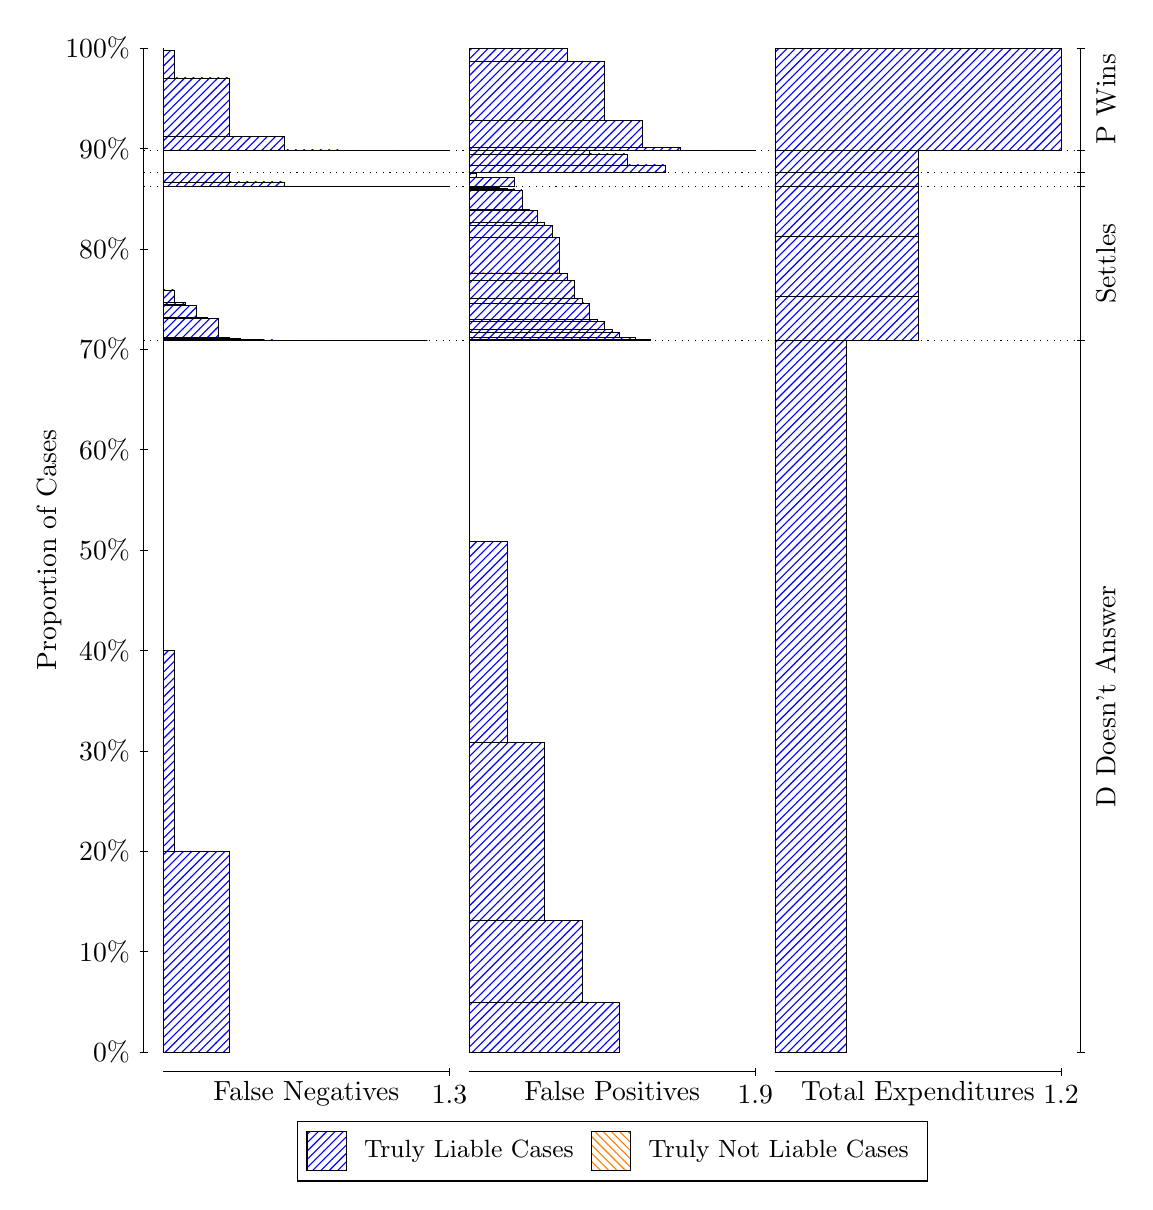
\begin{tikzpicture}
\draw[black, very thin] (1.5,1.75) -- (1.5,14.5);
\node[rotate=90, anchor=center] at (0.3, 8.125) {Proportion of Cases};
\draw[black, very thin] (1.45,1.75) -- (1.55,1.75);
\node[anchor=east] at (1.45, 1.75) {0\%};
\draw[black, very thin] (1.45,3.025) -- (1.55,3.025);
\node[anchor=east] at (1.45, 3.025) {10\%};
\draw[black, very thin] (1.45,4.3) -- (1.55,4.3);
\node[anchor=east] at (1.45, 4.3) {20\%};
\draw[black, very thin] (1.45,5.575) -- (1.55,5.575);
\node[anchor=east] at (1.45, 5.575) {30\%};
\draw[black, very thin] (1.45,6.85) -- (1.55,6.85);
\node[anchor=east] at (1.45, 6.85) {40\%};
\draw[black, very thin] (1.45,8.125) -- (1.55,8.125);
\node[anchor=east] at (1.45, 8.125) {50\%};
\draw[black, very thin] (1.45,9.4) -- (1.55,9.4);
\node[anchor=east] at (1.45, 9.4) {60\%};
\draw[black, very thin] (1.45,10.675) -- (1.55,10.675);
\node[anchor=east] at (1.45, 10.675) {70\%};
\draw[black, very thin] (1.45,11.95) -- (1.55,11.95);
\node[anchor=east] at (1.45, 11.95) {80\%};
\draw[black, very thin] (1.45,13.225) -- (1.55,13.225);
\node[anchor=east] at (1.45, 13.225) {90\%};
\draw[black, very thin] (1.45,14.5) -- (1.55,14.5);
\node[anchor=east] at (1.45, 14.5) {100\%};

\draw[black, very thin] (13.4,1.75) -- (13.4,14.5);
\draw[black, very thin] (13.35,1.75) -- (13.45,1.75);
\node[anchor=west] at (13.35, 1.75) {};
\draw[black, very thin] (13.35,10.783) -- (13.45,10.783);
\node[anchor=west] at (13.35, 10.783) {};
\draw[black, very thin] (13.35,12.739) -- (13.45,12.739);
\node[anchor=west] at (13.35, 12.739) {};
\draw[black, very thin] (13.35,12.918) -- (13.45,12.918);
\node[anchor=west] at (13.35, 12.918) {};
\draw[black, very thin] (13.35,13.203) -- (13.45,13.203);
\node[anchor=west] at (13.35, 13.203) {};
\draw[black, very thin] (13.35,14.5) -- (13.45,14.5);
\node[anchor=west] at (13.35, 14.5) {};

\draw[black, very thin, pattern color=blue, pattern=north east lines] (1.75,1.75) rectangle (2.5885,4.2999);
\draw[black, very thin, pattern color=blue, pattern=north east lines] (1.75,4.2999) rectangle (1.8897,6.8475);
\draw[black, very thin, pattern color=orange, pattern=north west lines] (1.75,6.8475) rectangle (1.75,6.8475);
\draw[black, very thin, pattern color=blue, pattern=north east lines] (1.75,6.8475) rectangle (1.75,10.783);
\draw[black, very thin, pattern color=blue, pattern=north east lines] (1.75,10.783) rectangle (5.1038,10.783);
\draw[black, very thin, pattern color=blue, pattern=north east lines] (1.75,10.783) rectangle (4.8244,10.783);
\draw[black, very thin, pattern color=blue, pattern=north east lines] (1.75,10.783) rectangle (4.5449,10.783);
\draw[black, very thin, pattern color=blue, pattern=north east lines] (1.75,10.783) rectangle (4.4051,10.783);
\draw[black, very thin, pattern color=blue, pattern=north east lines] (1.75,10.783) rectangle (4.2654,10.783);
\draw[black, very thin, pattern color=blue, pattern=north east lines] (1.75,10.783) rectangle (4.2654,10.783);
\draw[black, very thin, pattern color=blue, pattern=north east lines] (1.75,10.783) rectangle (4.1256,10.783);
\draw[black, very thin, pattern color=blue, pattern=north east lines] (1.75,10.783) rectangle (3.9859,10.783);
\draw[black, very thin, pattern color=blue, pattern=north east lines] (1.75,10.783) rectangle (3.8462,10.783);
\draw[black, very thin, pattern color=blue, pattern=north east lines] (1.75,10.783) rectangle (3.7064,10.784);
\draw[black, very thin, pattern color=blue, pattern=north east lines] (1.75,10.784) rectangle (3.5667,10.784);
\draw[black, very thin, pattern color=blue, pattern=north east lines] (1.75,10.784) rectangle (3.5667,10.784);
\draw[black, very thin, pattern color=blue, pattern=north east lines] (1.75,10.784) rectangle (3.4269,10.784);
\draw[black, very thin, pattern color=blue, pattern=north east lines] (1.75,10.784) rectangle (3.4269,10.784);
\draw[black, very thin, pattern color=blue, pattern=north east lines] (1.75,10.784) rectangle (3.2872,10.785);
\draw[black, very thin, pattern color=blue, pattern=north east lines] (1.75,10.785) rectangle (3.1474,10.793);
\draw[black, very thin, pattern color=blue, pattern=north east lines] (1.75,10.793) rectangle (3.0077,10.794);
\draw[black, very thin, pattern color=blue, pattern=north east lines] (1.75,10.794) rectangle (3.0077,10.795);
\draw[black, very thin, pattern color=blue, pattern=north east lines] (1.75,10.795) rectangle (2.8679,10.796);
\draw[black, very thin, pattern color=blue, pattern=north east lines] (1.75,10.796) rectangle (2.8679,10.801);
\draw[black, very thin, pattern color=blue, pattern=north east lines] (1.75,10.801) rectangle (2.8679,10.801);
\draw[black, very thin, pattern color=blue, pattern=north east lines] (1.75,10.801) rectangle (2.7282,10.802);
\draw[black, very thin, pattern color=blue, pattern=north east lines] (1.75,10.802) rectangle (2.7282,10.812);
\draw[black, very thin, pattern color=blue, pattern=north east lines] (1.75,10.812) rectangle (2.5885,10.824);
\draw[black, very thin, pattern color=blue, pattern=north east lines] (1.75,10.824) rectangle (2.4487,11.071);
\draw[black, very thin, pattern color=blue, pattern=north east lines] (1.75,11.071) rectangle (2.309,11.077);
\draw[black, very thin, pattern color=blue, pattern=north east lines] (1.75,11.077) rectangle (2.309,11.08);
\draw[black, very thin, pattern color=blue, pattern=north east lines] (1.75,11.08) rectangle (2.1692,11.084);
\draw[black, very thin, pattern color=blue, pattern=north east lines] (1.75,11.084) rectangle (2.1692,11.233);
\draw[black, very thin, pattern color=blue, pattern=north east lines] (1.75,11.233) rectangle (2.1692,11.233);
\draw[black, very thin, pattern color=blue, pattern=north east lines] (1.75,11.233) rectangle (2.0295,11.248);
\draw[black, very thin, pattern color=blue, pattern=north east lines] (1.75,11.248) rectangle (2.0295,11.27);
\draw[black, very thin, pattern color=blue, pattern=north east lines] (1.75,11.27) rectangle (1.8897,11.428);
\draw[black, very thin, pattern color=orange, pattern=north west lines] (1.75,11.428) rectangle (1.75,11.428);
\draw[black, very thin, pattern color=blue, pattern=north east lines] (1.75,11.428) rectangle (1.75,12.739);
\draw[black, very thin, pattern color=blue, pattern=north east lines] (1.75,12.739) rectangle (5.3833,12.739);
\draw[black, very thin, pattern color=blue, pattern=north east lines] (1.75,12.739) rectangle (4.6846,12.739);
\draw[black, very thin, pattern color=blue, pattern=north east lines] (1.75,12.739) rectangle (3.9859,12.744);
\draw[black, very thin, pattern color=blue, pattern=north east lines] (1.75,12.744) rectangle (3.2872,12.8);
\draw[black, very thin, pattern color=blue, pattern=north east lines] (1.75,12.8) rectangle (2.5885,12.918);
\draw[black, very thin, pattern color=orange, pattern=north west lines] (1.75,12.918) rectangle (1.75,12.918);
\draw[black, very thin, pattern color=blue, pattern=north east lines] (1.75,12.918) rectangle (2.5885,12.918);
\draw[black, very thin, pattern color=blue, pattern=north east lines] (1.75,12.918) rectangle (1.8897,12.918);
\draw[black, very thin, pattern color=orange, pattern=north west lines] (1.75,12.918) rectangle (1.75,12.918);
\draw[black, very thin, pattern color=blue, pattern=north east lines] (1.75,12.918) rectangle (1.75,13.203);
\draw[black, very thin, pattern color=blue, pattern=north east lines] (1.75,13.203) rectangle (5.3833,13.203);
\draw[black, very thin, pattern color=blue, pattern=north east lines] (1.75,13.203) rectangle (4.6846,13.203);
\draw[black, very thin, pattern color=blue, pattern=north east lines] (1.75,13.203) rectangle (3.9859,13.207);
\draw[black, very thin, pattern color=blue, pattern=north east lines] (1.75,13.207) rectangle (3.2872,13.375);
\draw[black, very thin, pattern color=blue, pattern=north east lines] (1.75,13.375) rectangle (2.5885,13.375);
\draw[black, very thin, pattern color=blue, pattern=north east lines] (1.75,13.375) rectangle (2.5885,14.12);
\draw[black, very thin, pattern color=blue, pattern=north east lines] (1.75,14.12) rectangle (1.8897,14.12);
\draw[black, very thin, pattern color=blue, pattern=north east lines] (1.75,14.12) rectangle (1.8897,14.466);
\draw[black, very thin, pattern color=orange, pattern=north west lines] (1.75,14.466) rectangle (1.75,14.466);
\draw[black, very thin, pattern color=blue, pattern=north east lines] (1.75,14.466) rectangle (1.75,14.5);
\draw[black, very thin, pattern color=orange, pattern=north west lines] (5.6333,1.75) rectangle (7.5456,1.75);
\draw[black, very thin, pattern color=blue, pattern=north east lines] (5.6333,1.75) rectangle (7.5456,2.3828);
\draw[black, very thin, pattern color=blue, pattern=north east lines] (5.6333,2.3828) rectangle (7.0675,3.4165);
\draw[black, very thin, pattern color=blue, pattern=north east lines] (5.6333,3.4165) rectangle (6.5895,5.6858);
\draw[black, very thin, pattern color=blue, pattern=north east lines] (5.6333,5.6858) rectangle (6.1114,8.2335);
\draw[black, very thin, pattern color=blue, pattern=north east lines] (5.6333,8.2335) rectangle (5.6333,10.783);
\draw[black, very thin, pattern color=orange, pattern=north west lines] (5.6333,10.783) rectangle (7.9281,10.783);
\draw[black, very thin, pattern color=blue, pattern=north east lines] (5.6333,10.783) rectangle (7.9281,10.803);
\draw[black, very thin, pattern color=orange, pattern=north west lines] (5.6333,10.803) rectangle (7.7368,10.803);
\draw[black, very thin, pattern color=blue, pattern=north east lines] (5.6333,10.803) rectangle (7.7368,10.825);
\draw[black, very thin, pattern color=orange, pattern=north west lines] (5.6333,10.825) rectangle (7.5456,10.825);
\draw[black, very thin, pattern color=blue, pattern=north east lines] (5.6333,10.825) rectangle (7.5456,10.892);
\draw[black, very thin, pattern color=blue, pattern=north east lines] (5.6333,10.892) rectangle (7.45,10.923);
\draw[black, very thin, pattern color=orange, pattern=north west lines] (5.6333,10.923) rectangle (7.3544,10.923);
\draw[black, very thin, pattern color=blue, pattern=north east lines] (5.6333,10.923) rectangle (7.3544,11.033);
\draw[black, very thin, pattern color=blue, pattern=north east lines] (5.6333,11.033) rectangle (7.2588,11.054);
\draw[black, very thin, pattern color=orange, pattern=north west lines] (5.6333,11.054) rectangle (7.1632,11.054);
\draw[black, very thin, pattern color=blue, pattern=north east lines] (5.6333,11.054) rectangle (7.1632,11.262);
\draw[black, very thin, pattern color=blue, pattern=north east lines] (5.6333,11.262) rectangle (7.0675,11.321);
\draw[black, very thin, pattern color=orange, pattern=north west lines] (5.6333,11.321) rectangle (6.9719,11.321);
\draw[black, very thin, pattern color=blue, pattern=north east lines] (5.6333,11.321) rectangle (6.9719,11.552);
\draw[black, very thin, pattern color=blue, pattern=north east lines] (5.6333,11.552) rectangle (6.8763,11.637);
\draw[black, very thin, pattern color=blue, pattern=north east lines] (5.6333,11.637) rectangle (6.7807,11.643);
\draw[black, very thin, pattern color=orange, pattern=north west lines] (5.6333,11.643) rectangle (6.7807,11.643);
\draw[black, very thin, pattern color=blue, pattern=north east lines] (5.6333,11.643) rectangle (6.7807,12.094);
\draw[black, very thin, pattern color=blue, pattern=north east lines] (5.6333,12.094) rectangle (6.6851,12.252);
\draw[black, very thin, pattern color=orange, pattern=north west lines] (5.6333,12.252) rectangle (6.5895,12.252);
\draw[black, very thin, pattern color=blue, pattern=north east lines] (5.6333,12.252) rectangle (6.5895,12.289);
\draw[black, very thin, pattern color=blue, pattern=north east lines] (5.6333,12.289) rectangle (6.4939,12.442);
\draw[black, very thin, pattern color=orange, pattern=north west lines] (5.6333,12.442) rectangle (6.3982,12.442);
\draw[black, very thin, pattern color=blue, pattern=north east lines] (5.6333,12.442) rectangle (6.3982,12.445);
\draw[black, very thin, pattern color=blue, pattern=north east lines] (5.6333,12.445) rectangle (6.3982,12.451);
\draw[black, very thin, pattern color=blue, pattern=north east lines] (5.6333,12.451) rectangle (6.3026,12.451);
\draw[black, very thin, pattern color=blue, pattern=north east lines] (5.6333,12.451) rectangle (6.3026,12.698);
\draw[black, very thin, pattern color=blue, pattern=north east lines] (5.6333,12.698) rectangle (6.207,12.71);
\draw[black, very thin, pattern color=blue, pattern=north east lines] (5.6333,12.71) rectangle (6.1114,12.721);
\draw[black, very thin, pattern color=blue, pattern=north east lines] (5.6333,12.721) rectangle (6.0158,12.727);
\draw[black, very thin, pattern color=blue, pattern=north east lines] (5.6333,12.727) rectangle (5.9202,12.729);
\draw[black, very thin, pattern color=blue, pattern=north east lines] (5.6333,12.729) rectangle (5.9202,12.729);
\draw[black, very thin, pattern color=blue, pattern=north east lines] (5.6333,12.729) rectangle (5.8246,12.729);
\draw[black, very thin, pattern color=blue, pattern=north east lines] (5.6333,12.729) rectangle (5.8246,12.738);
\draw[black, very thin, pattern color=blue, pattern=north east lines] (5.6333,12.738) rectangle (5.7289,12.738);
\draw[black, very thin, pattern color=blue, pattern=north east lines] (5.6333,12.738) rectangle (5.6333,12.739);
\draw[black, very thin, pattern color=orange, pattern=north west lines] (5.6333,12.739) rectangle (6.207,12.739);
\draw[black, very thin, pattern color=blue, pattern=north east lines] (5.6333,12.739) rectangle (6.207,12.856);
\draw[black, very thin, pattern color=blue, pattern=north east lines] (5.6333,12.856) rectangle (5.7289,12.913);
\draw[black, very thin, pattern color=blue, pattern=north east lines] (5.6333,12.913) rectangle (5.6333,12.918);
\draw[black, very thin, pattern color=orange, pattern=north west lines] (5.6333,12.918) rectangle (8.1193,12.918);
\draw[black, very thin, pattern color=blue, pattern=north east lines] (5.6333,12.918) rectangle (8.1193,13.016);
\draw[black, very thin, pattern color=blue, pattern=north east lines] (5.6333,13.016) rectangle (7.6412,13.157);
\draw[black, very thin, pattern color=blue, pattern=north east lines] (5.6333,13.157) rectangle (7.1632,13.202);
\draw[black, very thin, pattern color=blue, pattern=north east lines] (5.6333,13.202) rectangle (6.6851,13.203);
\draw[black, very thin, pattern color=blue, pattern=north east lines] (5.6333,13.203) rectangle (6.207,13.203);
\draw[black, very thin, pattern color=orange, pattern=north west lines] (5.6333,13.203) rectangle (9.2667,13.203);
\draw[black, very thin, pattern color=blue, pattern=north east lines] (5.6333,13.203) rectangle (9.2667,13.203);
\draw[black, very thin, pattern color=orange, pattern=north west lines] (5.6333,13.203) rectangle (8.7886,13.203);
\draw[black, very thin, pattern color=blue, pattern=north east lines] (5.6333,13.203) rectangle (8.7886,13.203);
\draw[black, very thin, pattern color=orange, pattern=north west lines] (5.6333,13.203) rectangle (8.3105,13.203);
\draw[black, very thin, pattern color=blue, pattern=north east lines] (5.6333,13.203) rectangle (8.3105,13.237);
\draw[black, very thin, pattern color=orange, pattern=north west lines] (5.6333,13.237) rectangle (7.8325,13.237);
\draw[black, very thin, pattern color=blue, pattern=north east lines] (5.6333,13.237) rectangle (7.8325,13.583);
\draw[black, very thin, pattern color=orange, pattern=north west lines] (5.6333,13.583) rectangle (7.3544,13.583);
\draw[black, very thin, pattern color=blue, pattern=north east lines] (5.6333,13.583) rectangle (7.3544,14.328);
\draw[black, very thin, pattern color=blue, pattern=north east lines] (5.6333,14.328) rectangle (6.8763,14.496);
\draw[black, very thin, pattern color=blue, pattern=north east lines] (5.6333,14.496) rectangle (6.3982,14.5);
\draw[black, very thin, pattern color=blue, pattern=north east lines] (5.6333,14.5) rectangle (5.9202,14.5);
\draw[black, very thin, pattern color=blue, pattern=north east lines] (5.6333,14.5) rectangle (5.6333,14.5);
\draw[black, very thin, pattern color=orange, pattern=north west lines] (9.5167,1.75) rectangle (10.425,1.75);
\draw[black, very thin, pattern color=blue, pattern=north east lines] (9.5167,1.75) rectangle (10.425,10.783);
\draw[black, very thin, pattern color=orange, pattern=north west lines] (9.5167,10.783) rectangle (11.333,10.783);
\draw[black, very thin, pattern color=blue, pattern=north east lines] (9.5167,10.783) rectangle (11.333,11.35);
\draw[black, very thin, pattern color=orange, pattern=north west lines] (9.5167,11.35) rectangle (11.333,11.35);
\draw[black, very thin, pattern color=blue, pattern=north east lines] (9.5167,11.35) rectangle (11.333,12.106);
\draw[black, very thin, pattern color=orange, pattern=north west lines] (9.5167,12.106) rectangle (11.333,12.106);
\draw[black, very thin, pattern color=blue, pattern=north east lines] (9.5167,12.106) rectangle (11.333,12.739);
\draw[black, very thin, pattern color=orange, pattern=north west lines] (9.5167,12.739) rectangle (11.333,12.739);
\draw[black, very thin, pattern color=blue, pattern=north east lines] (9.5167,12.739) rectangle (11.333,12.918);
\draw[black, very thin, pattern color=orange, pattern=north west lines] (9.5167,12.918) rectangle (11.333,12.918);
\draw[black, very thin, pattern color=blue, pattern=north east lines] (9.5167,12.918) rectangle (11.333,13.203);
\draw[black, very thin, pattern color=orange, pattern=north west lines] (9.5167,13.203) rectangle (13.15,13.203);
\draw[black, very thin, pattern color=blue, pattern=north east lines] (9.5167,13.203) rectangle (13.15,14.5);
\draw[black, dotted] (1.5,10.783) -- (13.4,10.783);
\draw[black, dotted] (1.5,12.739) -- (13.4,12.739);
\draw[black, dotted] (1.5,12.918) -- (13.4,12.918);
\draw[black, dotted] (1.5,13.203) -- (13.4,13.203);
\draw[black, very thin] (1.75,1.5) -- (5.3833,1.5);
\node[anchor=north] at (3.5667, 1.5) {False Negatives};
\draw[black, very thin] (5.3833,1.45) -- (5.3833,1.55);
\node[anchor=north] at (5.3833, 1.45) {1.3};

\draw[black, very thin] (5.6333,1.5) -- (9.2667,1.5);
\node[anchor=north] at (7.45, 1.5) {False Positives};
\draw[black, very thin] (9.2667,1.45) -- (9.2667,1.55);
\node[anchor=north] at (9.2667, 1.45) {1.9};

\draw[black, very thin] (9.5167,1.5) -- (13.15,1.5);
\node[anchor=north] at (11.333, 1.5) {Total Expenditures};
\draw[black, very thin] (13.15,1.45) -- (13.15,1.55);
\node[anchor=north] at (13.15, 1.45) {1.2};

\node[black, centered, rotate=90] at (13.72, 6.2667) {D Doesn't Answer};
\node[black, centered, rotate=90] at (13.72, 11.761) {Settles};


\node[black, centered, rotate=90] at (13.72, 13.851) {P Wins};

\draw (7.449999999999999,1.5) node[draw=none] (baseCoordinate) {};
\begin{scope}[align=center]
        \matrix[scale=0.5, draw=black, below=0.5cm of baseCoordinate, nodes={draw}, column sep=0.1cm]{
            \node[rectangle, draw, minimum width=0.5cm, minimum height=0.5cm, pattern=north east lines, pattern color=blue] {}; &
            \node[draw=none, font=\small] (B) {Truly Liable Cases}; &
            \node[rectangle, draw, minimum width=0.5cm, minimum height=0.5cm, pattern=north west lines, pattern color=orange] {}; &
            \node[draw=none, font=\small] (B) {Truly Not Liable Cases}; \\
            };
\end{scope}

\end{tikzpicture}
\end{document}